\section{Аналитическая часть}

\subsection{Гипертекстовые документы}

Гипертекстовым документом является документ, состоящий из текстовых страниц, имеющих перекрёстные ссылки. 
В данной работе под гипертекстовыми документами будут подразумеваться документы, написанные при помощи языка гипертекстовой разметки (англ. \textit{HyperText Markup Language} --- HTML) \cite{html}, а именно документы, соблюдающие стандарт HTML5 \cite{html-doc}.


Данный выбор обусловлен тем, что использование HTML5 получило широкое распространение в Всемирной сети благодаря рекомендации \cite{html-recommendation} к использованию от Консорциума Всемирной паутины (англ. \textit{World Wide Web Consortium} --- W3C).
Вследствие данной рекомендации HTML документы поддерживают большинство самых распространённых браузеров в России, такие, как Google Chrome, Яндекс.Браузер и Safari. 

\subsection{Объектная модель документа}
Объектная модель документа (англ. \textit{Document Object Model} --- DOM) \cite{dom} --- программный интерфейс для HTML, XML и CSV документов. 
Он обеспечивает структурированное представление документа (дерева), и определяет способ, по которому структура может быть доступна для программы, для изменения структуры документа, его стиля и содержания.
Представление DOM состоит из структурированной группы узлов и объектов, которые имеют свойства и методы.

Стадарт W3C DOM \cite{dom-doc} формирует основы DOM, реализованные в большинстве современных браузеров. 
Многие браузеры предлагают расширения за пределами данного стандарта, поэтому необходимо проверять работоспособность тех или иных возможностей DOM для каждого конкретного браузера.

Для описания структуры DOM потребуются следующие термины: корневой, родительские и дочерние элементы. 
Корневой элемент находится в основании всей структуры и не имеет родительского элемента.
Дочерние элементы не просто находятся внутри родительских, но и наследуют различные свойства от них.
Рассмотрим, как выглядит DOM-представление следующего HTML документа. 

\begin{code}
	\captionof{listing}{Пример простого HTML документа}
	\label{code:1}
	\inputminted
	[
	frame=single,
	framerule=0.5pt,
	framesep=20pt,
	fontsize=\small,
	tabsize=4,
	linenos,
	numbersep=5pt,
	xleftmargin=10pt,
	]
	{text}
	{code/simple.html}
\end{code}

Корневым элементом здесь является \textit{html}, он не имеет родительского элемента и имеет два дочерних --- \textit{head} и \textit{body}. По отношению друг к другу элементы \textit{head} и \textit{body} являются сиблингами (братьями и сестрами). В каждый из них можно вложить еще много дочерних элементов. Например, в head обычно находятся \textit{link}, \textit{meta}, \textit{script} или \textit{title}.

Данный HTML документ будет иметь следующее DOM-представление:
 \clearpage

\begin{figure}[h]
	\centering
	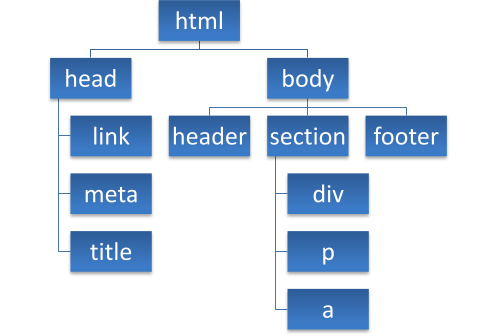
\includegraphics[width=150mm]{img/simple-dom-1.png}
	\caption{Пример DOM-представления для простого HTML документа}
	\label{fig:simple-dom-1}
\end{figure}

Все эти теги не являются уникальными, и в одном документе может быть по несколько экземпляров каждого из них.

В \textit{body} могут находиться разнообразные элементы. 
Например, в родительском \textit{body} --- дочерний элемент \textit{header}, в элементе \textit{header} --- дочерний элемент section, в родительском section --- дочерний \textit{div}, в \textit{div} --- элемент \textit{h3}, и, наконец, в \textit{h3} — элемент \textit{span}. 
В этом случае \textit{span} не имеет дочерних элементов, но их можно добавить в любой момент.
Это можно описать так:

\begin{figure}[h]
	\centering
	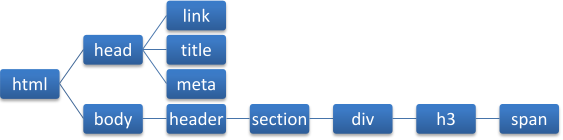
\includegraphics[width=\textwidth]{img/simple-dom-2.png}
	\caption{Пример DOM-представления для чуть более сложного HTML документа}
	\label{fig:simple-dom-2}
\end{figure}

\clearpage

А если бы система была бы более разветвлённая и с большим количеством вложений --- так:

\begin{figure}[h]
	\centering
	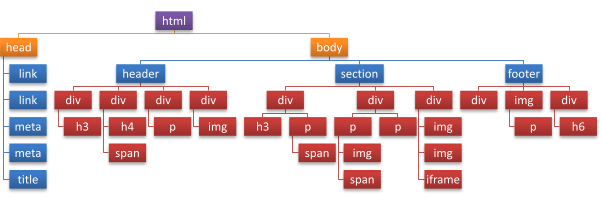
\includegraphics[width=150mm]{img/complicated-dom.png}
	\caption{Пример DOM-представления для сложного HTML документа}
	\label{fig:complicated-dom}
\end{figure}

На схеме изображено довольно большое DOM-дерево, и его сложно воспринимать из-за его размера.
Для удобства часто используется система многоуровневых списков. 
Например, предыдущее дерево можно преобразовать в такой список:

\begin{figure}[h]
	\centering
	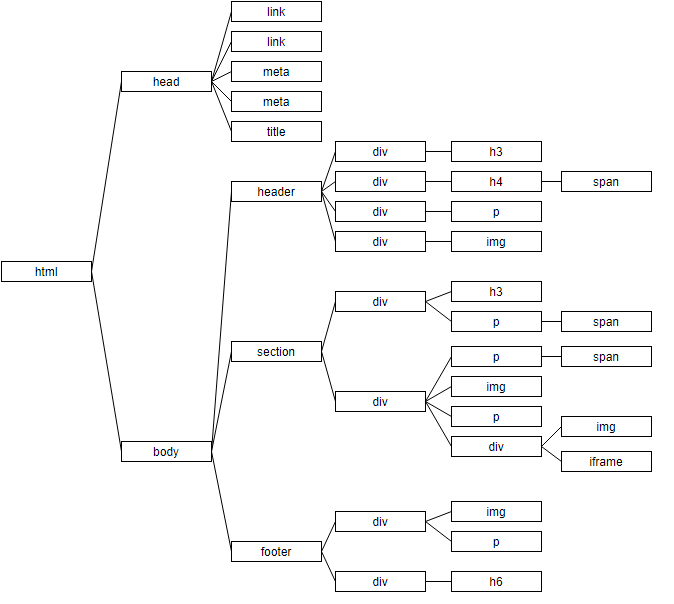
\includegraphics[width=150mm]{img/complicated-dom-list.png}
	\caption{Пример DOM-представления для сложного HTML документа в виде списка}
	\label{fig:complicated-dom-list}
\end{figure}

\clearpage

Элементы могут наследовать не все, но многие свойства своих родителей --- например, цвет, шрифт, видимость, размеры и т.д.

Таким образом, чтобы задать стиль шрифта на всей странице, потребуется не прописывать цвет для каждого элемента, а задать его только для body. 
А чтобы изменить наследуемое свойство у дочернего элемента, нужно прописать только ему новые свойства. 
Наследование удобно для создания единообразной страницы.


\subsubsection{Алгоритм построения DOM}

Рассмотрим алгоритм построения DOM-дерева по имеющемуся HTML документу.

Для того, чтобы построить дерево объектной модели, требуется обработать документ и произвести операцию вставки в получающееся дерево $n$ раз, где $n$ - количество элементов.

\subsubsection{Алгоритм отображения DOM}

Полученное DOM-дерево необходимо отобразить, чтобы пользователь получил возможность увидеть результаты отображения у себя на экране.

Чтобы это сделать, придётся сделать полный обход DOM-дерева и отобразить каждый из имеющихся элементов.

\subsubsection{Алгоритм обновления DOM}

Обновление структуры DOM --- распространённая и часто используемая операция, производимая, например, в случае, когда документ должен меняться в ответ на действия пользователя (любая активность на странице).

Рекоммендация W3C в таком случае призывает повторно отрисовать обновлённое дерево с нуля --- то есть, каждый раз, когда необходимо обновить дерево, будет использоваться алгоритм отображения.

\clearpage

\subsection{Виртуальная объектная модель документа}

